
\subsection{Run and Event Selection}

% total number of runs containing triggered events

% -- so many runs get tossed out, though

% describe QA checks
% - use the best reconstructed vertex for the event.  If no vertex was reconstructed, skip the event
% - identified spin states for the colliding bunches in both beams
% - vertex position from scaler timing information falls within a window

% list numbers of runs that survive those checks, as well as corresponding sampled luminosity

\subsection{Pion Identification}

Charged pions are identified from the subset of primary tracks in each event
having at least 25 fit points, a distance of closest approach (DCA) to the
primary vertex of no more than 1 centimeter, a pseudorapidity magnitude less
than 1.0, and a transverse momentum greater than 2.0 GeV/c. The first three cuts
select high quality tracks. The transverse momentum cut is not necessary from an
experimental perspective, but an \(A_{LL}\) analysis of low momentum pions
offers limited physics insights and the analysis can proceed more efficiently if
these very common particles are not included. The determination of the PID
acceptance window is discussed in Section~\ref{sec:pid} and the window
boundaries are listed in Table~\ref{tbl:pid-selection-windows}.
Figure~\ref{fig:pid-accept-window} highlights the characteristic MIP
distribution of the accepted charged pion tracks.

% TODO drift velocity fix?  cool to include, since I did it. Not needed though

\begin{table}
  \centering
  \begin{tabular}{|c|c|}
    \hline
    Criterion & Efficiency \\
    \hline
    $|\eta| < 1.0$ & 0.94 \\
    at least 25 fit points & 0.95 \\
    $|DCA|$ of associated global track $<$ 1.0 cm & 0.96 \\
    \hline
  \end{tabular}
  \caption{Quality cuts imposed on the high-$p_T$ primary tracks before PID selection.}
\end{table}

\begin{figure}
  \centering
  \includegraphics[width=0.5\textwidth]{figures/placeholder}
  \caption{Energy loss per unit path length versus momentum for tracks produced by identified charged pions.}
  \label{fig:pid-accept-window}
\end{figure}

\subsection{Jet-Pion Correlations}

% TODO description of QA procedure? (essentially jet QA)

In the 2006 data analysis events are accepted only if they contain a
reconstructed jet with an uncorrected \(p_T\) between 10 and 30 GeV/c, a
pseudorapidity between -0.7 and 0.9, and an electromagnetic energy fraction not
greater than 0.92. Furthermore, the difference in azimuth between the jet axis
and the center of a jet patch above the trigger threshold must be no more than
\(36^\circ\). Multiple jets in an event can satisfy these ``trigger jet'' cuts.

Charged pions satisfying the track quality and PID cuts described in the
preceding section are compared against the list of trigger jets. If a charged
pion is separated from a trigger jet by at least 2.0 radians in azimuth it is
considered to be an ``away-side'' pion and is accepted for analysis.
Figure~\ref{fig:dphi} plots the azimuthal distribution of charged pions relative
to trigger jets in the 2006 analysis. The data show good agreement with Monte
Carlo simulations.

\begin{figure}
  \centering
  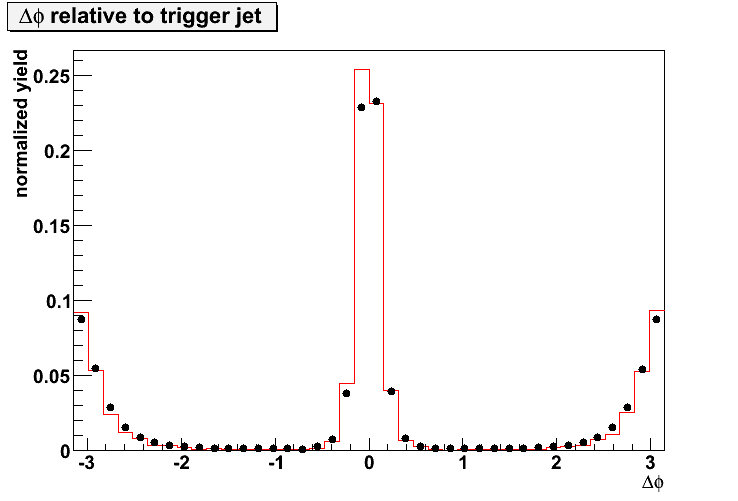
\includegraphics[width=0.7\textwidth]{figures/dphi}
  \caption{Azimuthal distribution of charged pions relative to the trigger jet axis in the 2006 dataset.  The black circles represent data, the red lines fully reconstructed Monte Carlo. Pions with $|\Delta \phi| > 2.0$ are accepted for analysis.}
  \label{fig:dphi}
\end{figure}

The data are binned as a function of \(z\), defined as the ratio of the
away-side pion \(p_T\) and the trigger jet \(p_T\). Figure~\ref{fig:meanpt}
shows that the jet \(\langle p_T \rangle\) is approximately constant as a
function of \(z\), and thus that the charged pion \(\langle p_T \rangle\)
increases linearly with \(z\). Again, the data are modeled well by STAR's
Pythia+GEANT simulations.

\begin{figure}
  \centering
  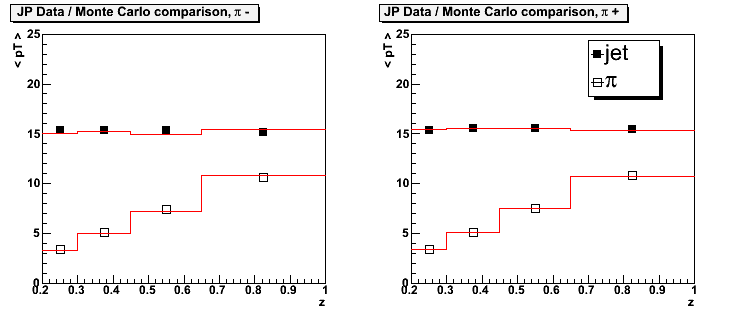
\includegraphics[width=1.0\textwidth]{figures/meanpt}
  \caption{Comparison of the $\langle p_T \rangle$ values for jets and charged pions in each $z$ bin.  The data show good agreement with fully reconstructed Pythia+GEANT events that pass a simulation of the BJP2 trigger.}
  \label{fig:meanpt}
\end{figure}
